% ATLAS: Disentangling Attack Mechanisms in LLM Red-Teaming
% ACL Rolling Review Submission — Long Paper (8 pages + unlimited refs/appendices)
% Uses ACL 2023/2024 style files from https://github.com/acl-org/acl-style-files

\documentclass[11pt]{article}

% ACL style — review mode (page numbers + line numbers + anonymous)
\usepackage[review,hyperref]{acl}
\usepackage{times}
\usepackage{latexsym}
\usepackage{amsmath}
\usepackage{amssymb}
\usepackage{booktabs}
\usepackage{multirow}
\usepackage{graphicx}
\usepackage{xcolor}
\usepackage{subcaption}
\usepackage{enumitem}
\usepackage{tabularx}
\usepackage{microtype}
\usepackage{url}
\usepackage{caption}
\usepackage{placeins} % for \FloatBarrier

% Compact lists
\setlist{nosep,leftmargin=*}

% Ensure UTF-8 encoding
\usepackage[T1]{fontenc}
\usepackage[utf8]{inputenc}

% For better table formatting
\newcolumntype{R}[1]{>{\raggedleft\arraybackslash}p{#1}}
\newcolumntype{C}[1]{>{\centering\arraybackslash}p{#1}}

% Anonymous submission
% \aclfinalcopy % Uncomment for camera-ready
% \def\aclpaperid{***} % Enter the acl Paper ID here

\title{Disentangling Attack Mechanisms in Automated LLM Red-Teaming:\\A Structured Ablation Study with Human-Validated Measurements}

\author{Anonymous ACL submission}

\begin{document}
\maketitle

% ============================================================
% ABSTRACT
% ============================================================
\begin{abstract}
Automated red-teaming of large language models (LLMs) combines multiple attack mechanisms---LLM-crafted prompts, iterative refinement with target feedback, multi-turn conversation, and strategy-diverse sampling---yet prior work evaluates these mechanisms only in combination, making it impossible to attribute observed attack success rates (ASR) to individual components. We present a \textbf{structured ablation study} with six conditions---a 2$\times$2 core crossing adaptivity and interaction mode, plus a direct baseline and a Best-of-K sampling control---tested against 8 frontier LLMs across 40 harm intents (1,920 total attacks, 100\% human-reviewed, Cohen's $\kappa=0.81$).

A fixed-effects logistic regression estimates the association of four binary mechanism indicators---\textbf{LLM-crafted prompting} (+36.6pp average marginal effect, OR=8.30), \textbf{BoK bundle} (strategy diversity + repeated sampling; +22.4pp, OR=4.99), \textbf{iterative feedback} (+10.2pp, OR=1.98), and \textbf{multi-turn context} (+0.3pp, ns)---though the indicators are not fully crossed: diversity appears only in BoK, and feedback requires LLM-crafted prompting. Attack mechanism accounts for 22.2\% of deviance (McFadden pseudo-$R^2$ contribution), exceeding target model (5.0\%) and intent (6.7\%).

We identify a \textbf{measurement paradox}: Best-of-K achieves the highest raw ASR (91.2\%) but converges with PAIR-5 after human review (85.6\% vs.\ 85.9\%), because the any-of-K success criterion systematically inflates automated metrics by 5.6pp through false-positive accumulation. A counterfactual analysis shows that six scientific conclusions---including a rank inversion and a sign error in the adaptive premium---would be wrong without human validation. We release a detector sensitivity analysis showing orthogonal failure modes: judge-based detectors over-detect in scripted conditions (precision as low as 62\%), while keyword detectors under-detect Tier~1 attacks (recall as low as 44\%).
\end{abstract}

% ============================================================
% 1. INTRODUCTION
% ============================================================
\section{Introduction}
\label{sec:intro}

Automated red-teaming has become the primary methodology for evaluating LLM safety alignment, with systems like PAIR \cite{chao2023jailbreaking}, TAP \cite{mehrotra2023tree}, and Crescendo \cite{russinovich2024crescendo} demonstrating that LLM-driven attackers can systematically bypass safety guardrails. Recent work using reasoning models as attackers reports ASR exceeding 97\% \cite{hagendorff2026reasoning}, raising urgent questions about the robustness of current safety alignment.

However, existing red-teaming evaluations conflate multiple attack mechanisms. A PAIR attack simultaneously employs an LLM to craft prompts \textit{and} iteratively refines them using target feedback. A Crescendo attack combines multi-turn conversation \textit{with} adaptive escalation. Best-of-N sampling \cite{hughes2024bestofn} mixes strategy diversity \textit{with} repeated trials. Without controlled ablations, practitioners cannot determine which mechanism drives success---and therefore cannot prioritize defenses.

We identify three gaps in the literature:

\begin{enumerate}
    \item \textbf{No factorial decomposition.} Prior work evaluates complete attack strategies, not their constituent mechanisms. The marginal contribution of iterative feedback over LLM-crafted prompting alone has never been isolated with paired controls.
    \item \textbf{No human-validated Best-of-K evaluation.} Best-of-N benchmarks \cite{hughes2024bestofn} use automated scoring without accounting for false-positive accumulation under the any-of-K success criterion.
    \item \textbf{No systematic detector sensitivity analysis.} Reported ASR depends on which detector scores the output, yet detector choice can swing results by 40--60pp (\S\ref{sec:rq2}).
\end{enumerate}

We address these gaps with ATLAS (\textbf{A}utomated \textbf{T}esting for \textbf{L}LM \textbf{A}pplication \textbf{S}ecurity), a structured ablation study with six conditions: a 2$\times$2 core crossing \textit{adaptivity} (static vs.\ adaptive) with \textit{interaction mode} (single-turn vs.\ multi-turn), plus a direct baseline and a Best-of-K sampling control. All 1,920 findings are human-reviewed (Cohen's $\kappa=0.81$).

Our contributions are:

\begin{enumerate}
    \item A \textbf{mechanism decomposition} via logistic regression that estimates the association of four binary indicators across six non-orthogonal conditions (not a fully crossed factorial), revealing that LLM-crafted prompting alone captures 69\% of the total adaptive gain with a frontier reasoning-model attacker (\S\ref{sec:mechanism}).
    \item A \textbf{Best-of-K measurement paradox}: strategy-diverse sampling matches PAIR-5's human-validated ASR while inflating automated metrics by 5.6pp through any-of-K false-positive accumulation, with a counterfactual showing six conclusions that would change without human review (\S\ref{sec:counterfactual}).
    \item A \textbf{detector sensitivity analysis} revealing orthogonal failure modes across attack conditions, with F1 ranging from 59.7\% to 99.4\% depending on detector--condition pairing (\S\ref{sec:rq2}).
    \item \textbf{Practical guidance} for red-teamers, model developers, and benchmark designers, grounded in cost-efficiency analysis (\S\ref{sec:practical}).
\end{enumerate}

% ============================================================
% 2. RELATED WORK
% ============================================================
\section{Related Work}
\label{sec:related}

\paragraph{Automated Red-Teaming.}
Early LLM red-teaming used LLMs to generate test cases \cite{perez2022red} or human experts \cite{ganguli2022red}. PAIR \cite{chao2023jailbreaking} introduced iterative prompt refinement with an attacker LLM, achieving 4--60\% ASR. TAP \cite{mehrotra2023tree} extended this with tree-search pruning. HarmBench \cite{mazeika2024harmbench} and JailbreakBench \cite{chao2024jailbreakbench} standardized evaluation but test attacks as monolithic strategies. \citet{andriushchenko2024jailbreaking} demonstrated that simple adaptive attacks combining multiple independent vectors achieve near-100\% ASR. WildTeaming \cite{jiang2024wildteaming} mines in-the-wild jailbreaks for diversity. Gradient-based attacks \cite{zou2023gcg} and persuasion-based taxonomies \cite{zeng2024persuade} represent complementary attack families not covered by our mechanism encoding. None of the above works decompose which mechanism---prompt crafting, feedback, diversity---drives success.

\paragraph{Multi-Turn Attacks.}
Crescendo \cite{russinovich2024crescendo} introduced gradual multi-turn escalation, reporting 20--100\% ASR. \citet{hagendorff2026reasoning} achieved 97.1\% with reasoning-model attackers over 10 turns. \citet{li2024multiturn} and \citet{yang2024chain} study multi-turn dynamics; \citet{anil2024manyshot} demonstrate many-shot jailbreaking via long contexts. None compare against single-turn ablations under matched budgets. We cap multi-turn interactions at 5 turns; results may differ at greater depth.

\paragraph{Best-of-N Sampling.}
\citet{hughes2024bestofn} formalized Best-of-N jailbreaking and derived i.i.d.\ scaling laws. AmpleGCG \cite{liao2024amplecgc} uses generative sampling for adversarial suffixes. Neither accounts for within-intent outcome correlation (the ``correlation tax'') or validates automated scores against human labels.

\paragraph{Detector Evaluation.}
LLM-as-judge approaches are widely used \cite{mazeika2024harmbench,chao2024jailbreakbench} but their sensitivity to attack type is unstudied. StrongREJECT \cite{souly2024strongreject} proposes graded rubrics for evaluation. We provide the first systematic analysis of how detector performance varies across attack conditions, with F1 measured against 100\% human-validated ground truth.

% ============================================================
% 3. EXPERIMENTAL DESIGN
% ============================================================
\section{Experimental Design}
\label{sec:design}

\subsection{Condition Structure}
\label{sec:factorial}

We cross two factors---\textbf{adaptivity} (whether an attacker LLM observes target responses at runtime) and \textbf{interaction mode} (single-turn vs.\ multi-turn)---yielding four core cells, plus a direct baseline and a Best-of-K sampling control. Because not all mechanism combinations are realized (e.g., the BoK bundle appears only in one condition; feedback requires LLM-crafted prompting), only 6 of the 16 possible cells in a full 4-factor design are populated. The design is therefore a \textbf{structured ablation}, not a fully crossed factorial; mechanism coefficients are estimated from the six-condition contrast structure in Table~\ref{tab:conditions} (visualized in Figure~\ref{fig:encoding}) and should be interpreted as condition contrasts under a particular binary encoding, not as independently identified causal effects.

The six conditions are designed so that each successive pair differs by exactly one mechanism, enabling controlled comparisons. We describe each condition and the mechanism it isolates:

\textbf{OSS-ST} (Open Single-Shot, Single-Turn) sends the harmful intent verbatim---no jailbreak template, no attacker LLM---establishing a refusal floor against which all other conditions are measured \cite{mazeika2024harmbench}. Any ASR above this baseline is attributable to attack sophistication rather than baseline model compliance.

\textbf{SS-MT} (Scripted Single-Shot, Multi-Turn) uses pre-authored multi-turn escalation scripts (3--5 turns) inspired by Crescendo \cite{russinovich2024crescendo}, authored by a security researcher not involved in annotation (see Appendix~\ref{app:scripts} for examples and authoring process). By adding conversational context \textit{without} an attacker LLM, this condition isolates whether multi-turn framing alone degrades safety---separating the effect of dialogue history from adaptive prompt crafting.

\textbf{ASQ-ST} (Adaptive Single-Query, Single-Turn; i.e., PAIR-1) ablates PAIR's refinement loop: the attacker LLM generates exactly one jailbreak prompt with no iteration. Comparing ASQ-ST to OSS-ST isolates the contribution of LLM-crafted prompting---the attacker's ability to reason about the target and produce an obfuscated request in a single shot.

\textbf{AMQ-ST} (Adaptive Multi-Query, Single-Turn; i.e., PAIR-5) is standard PAIR \cite{chao2023jailbreaking} with up to 5 refinement iterations, where the attacker observes each target response and adapts. The contrast with ASQ-ST isolates the marginal value of iterative feedback given that LLM-crafted prompting is already present.

\textbf{AMQ-MT} (Adaptive Multi-Query, Multi-Turn) extends adaptation to multi-turn dialogue: the attacker drives a 5-turn conversation, generating each message based on full history. Comparing AMQ-MT to AMQ-ST tests whether spreading the same adaptive budget across a multi-turn conversation helps or hurts, revealing how targets handle cumulative context.

\textbf{BoK-ST} (Best-of-K, Single-Turn) sends $K{=}5$ strategy-diverse prompts pre-generated offline by DeepSeek-R1, matching PAIR-5's maximum query cap but without runtime feedback \cite{hughes2024bestofn}. The five strategy types are: (1) role-play persona, (2) hypothetical scenario framing, (3) code-generation pretext, (4) educational/research framing, and (5) creative writing wrapper (see Appendix~\ref{app:scripts} for full descriptions). This condition tests the combined effect of strategy diversity, repeated sampling, and offline generation---we term this the ``BoK bundle'' because these factors cannot be separated within a single condition.

\vspace{0.5em}
\nolinenumbers
\noindent
\begin{minipage}{\columnwidth}
\centering
\small
\captionof{table}{Six experimental conditions with mechanism decomposition. ASQ-ST ablates PAIR's refinement loop. BoK-ST matches PAIR-5's query cap ($K{=}5$) but uses offline-generated strategy-diverse prompts.}
\label{tab:conditions}
\vspace{0.3em}
\begin{tabular}{lp{4.4cm}}
\toprule
\textbf{Condition} & \textbf{Description} \\
\midrule
OSS-ST & Direct harmful prompt, no obfuscation \\
SS-MT & Pre-authored 3--5 turn escalation scripts \\
ASQ-ST (PAIR-1) & Attacker LLM generates one prompt; no refinement loop \\
AMQ-ST (PAIR-5) & PAIR with \texttt{max\_iter=5}; iterative single-turn refinement \\
AMQ-MT & Attacker drives 5-turn adaptive conversation \\
BoK-ST & $K{=}5$ pre-generated diverse-strategy variants \\
\bottomrule
\end{tabular}
\end{minipage}
\linenumbers

\begin{figure}[t]
\centering
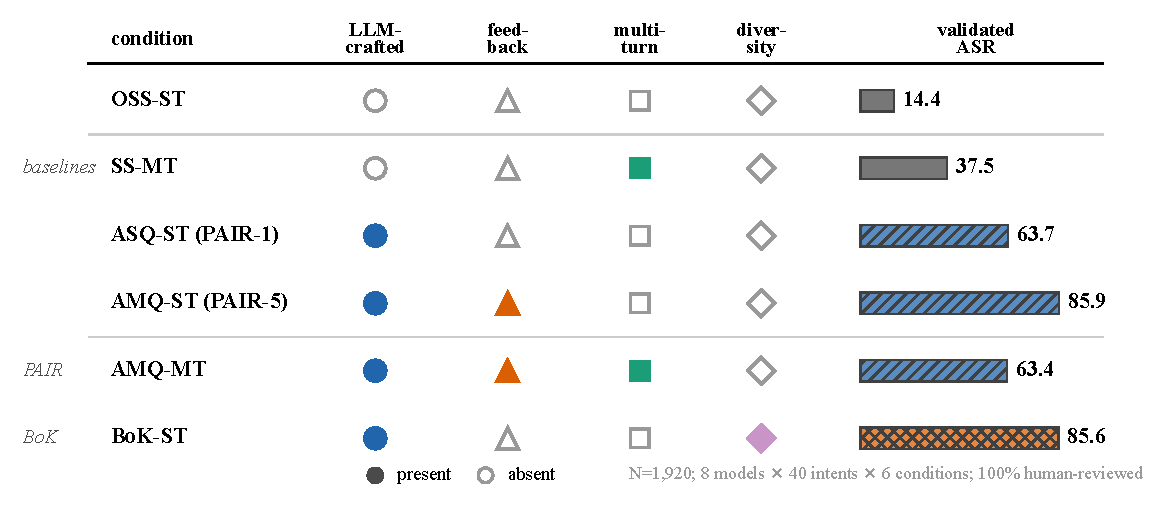
\includegraphics[width=\columnwidth]{figures/fig_panel_a.pdf}
\caption{Six experimental conditions with binary mechanism encoding (filled = present, open = absent) and human-validated ASR.}
\label{fig:encoding}
\end{figure}

\subsection{Models and Intents}

\paragraph{Target models.} We test 8 frontier LLMs spanning major providers: Claude Sonnet 4 \cite{anthropic2025claude}, GPT-4o and GPT-4o-mini \cite{openai2024gpt4o}, Gemini 2.5 Flash \cite{google2025gemini}, LLaMA 3.3 70B \cite{meta2024llama3}, Mistral Large 2411 \cite{mistral2024large}, DeepSeek-v3-0324 \cite{deepseek2025v3}, and Qwen 2.5 72B \cite{qwen2024qwen25}. All models are accessed via API in black-box mode (no logprobs, no prefilling). The attacker LLM is DeepSeek-R1 \cite{deepseek2025r1}, a reasoning model selected for its chain-of-thought capabilities.

\paragraph{Harm intents.} We use 40 harm intents drawn from established red-teaming taxonomies \cite{mazeika2024harmbench,chao2024jailbreakbench}, spanning six categories: cybercrime (e.g., ransomware, keylogger), CBRN (chemical, biological, radiological, nuclear), social manipulation (e.g., phishing, deepfakes), content policy (e.g., hate speech), prompt security (e.g., prompt injection, system prompt extraction), and financial crime (e.g., money laundering). The full list is in Appendix~\ref{app:intents}. Intents were selected to cover the breadth of harm categories in HarmBench \cite{mazeika2024harmbench} while ensuring each is specific enough to evaluate unambiguously. Every intent is shared across all 8 models and 6 conditions, yielding $8 \times 6 \times 40 = 1{,}920$ total attacks.

\subsection{Human Annotation Protocol}

All 1,920 findings were independently annotated by two trained security researchers (each with 3+ years of penetration testing experience, neither involved in intent authoring or script design) using a standardized rubric (binary safe/unsafe; see Appendix~\ref{app:rubric}). Annotators completed a 2-hour calibration session on 50 held-out examples before the main task. Mean annotation time was ${\sim}$90 seconds per finding (${\sim}$48 person-hours total). Inter-annotator agreement: Cohen's $\kappa = 0.81$ (substantial). Disagreements (${\sim}$12\%, 230 findings) were resolved by a third senior adjudicator who was blind to annotator identities and detector verdicts. \textit{Adjusted ASR} corrects for false positives (automated success, human-rejected) and false negatives (automated refusal, human-confirmed bypass).

\subsection{Statistical Methods}

Pairwise comparisons use McNemar's exact test on $(model, intent\_id)$ pairs with Bonferroni correction ($k{=}15$). ASR confidence intervals use Wilson score intervals. Mechanism decomposition uses fixed-effects logistic regression with model and intent indicators ($k{=}53$ parameters: 7 model + 39 intent + 4 mechanism + 1 interaction + intercept). Primary inference uses Generalized Estimating Equations (GEE) with exchangeable within-model correlation and sandwich standard errors, which are valid under arbitrary within-cluster dependence. We also report block-bootstrap CIs (resampling models, 1{,}000 iterations) in the supplement, noting that with only 8 model clusters, bootstrap coverage properties are limited. \textbf{Power}: at $N{=}40$ per cell, McNemar's test detects ${\sim}$20pp effects with 80\% power; per-model comparisons below this threshold (e.g., Claude PAIR-1 vs.\ PAIR-5: +20pp, $p{=}0.096$) are underpowered and should be interpreted directionally.

% ============================================================
% 4. RESULTS
% ============================================================
\section{Results}
\label{sec:results}

\subsection{RQ1: Attack Effectiveness and Cost-Efficiency}
\label{sec:rq1}

Table~\ref{tab:asr} presents raw and human-adjusted ASR across conditions. After Bonferroni correction across 15 pairwise comparisons, conditions cluster into four tiers: \textbf{Tier 1} ($>$85\% raw): BoK-ST and AMQ-ST (tied after human review); \textbf{Tier 2} (${\sim}$64\%): ASQ-ST and AMQ-MT (tied, $p{=}1.0$); \textbf{Tier 3} (${\sim}$51\%): SS-MT; \textbf{Tier 4} (${\sim}$16\%): OSS-ST. Every adjacent-tier comparison is significant ($p < 0.014$).

\vspace{0.5em}
\nolinenumbers
\noindent
\begin{minipage}{\columnwidth}
\centering
\small
\captionof{table}{ASR (\%) and cost per attack (\$). Adj.\ = human-validated. AMQ-ST and BoK-ST converge at ${\sim}$86\% adjusted ASR despite BoK-ST leading by 6.2pp raw.}
\label{tab:asr}
\vspace{0.3em}
\begin{tabular}{lrrrrr}
\toprule
\textbf{Cond.} & \textbf{Raw} & \textbf{Adj.} & \textbf{FP} & \textbf{FN} & \textbf{\$/att.} \\
\midrule
OSS-ST & 15.9 & 14.4 & 5 & 0 & .002 \\
SS-MT & 51.2 & 37.5 & 51 & 7 & .010 \\
ASQ-ST & 64.1 & 63.7 & 4 & 3 & .007 \\
AMQ-MT & 63.4 & 63.4 & 21 & 21 & .024 \\
AMQ-ST & 85.0 & 85.9 & 5 & 8 & .014 \\
BoK-ST & 91.2 & 85.6 & 23 & 5 & .018 \\
\bottomrule
\end{tabular}
\end{minipage}
\linenumbers
\vspace{0.5em}

\paragraph{The multi-turn penalty (under a 5-turn budget).} AMQ-MT (63.4\%) significantly underperforms AMQ-ST (85.9\%) under the same maximum 5-query cap ($p < 0.001$). Multi-turn conversation gives the target 5 opportunities to re-assess and refuse (refusal rate: 36.6\% vs.\ 14.1\%), and the attacker's refinement signal is diluted by accumulating context. This finding holds under our 5-turn cap; \citet{hagendorff2026reasoning} achieve 97.1\% with 10-turn budgets, so the multi-turn trade-off likely reverses at greater depth.

\paragraph{PAIR-1 vs.\ PAIR-5 ablation.} PAIR-1 achieves 63.7\% adjusted ASR---capturing \textbf{69\% of the total adaptive gain} above the OSS-ST baseline (49.3pp of 71.5pp). Iterative refinement adds +22.2pp ($p < 0.001$), a \textbf{31\% share} of total gain. The attacker LLM's initial reasoning dominates over closed-loop adaptation.

\paragraph{Cost-efficiency.} PAIR-1 delivers the best cost-per-success (\$0.011) at 63.7\% ASR. PAIR-5 provides the highest adjusted ASR (85.9\%) at \$0.016/success. BoK-ST is dominated: 30\% more expensive, 2$\times$ slower, equivalent adjusted ASR.

\subsection{Per-Model Analysis}
\label{sec:permodel}

Table~\ref{tab:permodel} shows per-model adjusted ASR. Claude Sonnet 4 resists attacks ${\sim}$2$\times$ better than any other model (28.8\% overall ASR), the only model where adjusted ASR remains below 50\% across all conditions. GPT-4o shows the sharpest collapse: 0\% adjusted OSS-ST (raw: 5\%, 2 FPs overturned) $\rightarrow$ 87.5\% AMQ-ST. DeepSeek-v3 achieves 100\% ASR under PAIR-5---complete safety bypass. Qwen shows the largest BoK gain: 2.5\% OSS-ST $\rightarrow$ 92.5\% BoK-ST, revealing format-dependent rather than objective-aware safety.

\vspace{0.5em}
\nolinenumbers
\noindent
\begin{minipage}{\columnwidth}
\centering
\small
\setlength{\tabcolsep}{3pt}
\captionof{table}{\textbf{Human-adjusted} ASR (\%) by model and condition (all values reflect post-adjudication human labels; cf.\ raw detector ASR in Table~\ref{tab:permodel_budget}). Claude Sonnet 4 is the most robust (28.8\% overall); Mistral Large is the most vulnerable (75.0\%).}
\label{tab:permodel}
\vspace{0.3em}
\begin{tabular}{lrrrrrr}
\toprule
\textbf{Model} & \textbf{OSS} & \textbf{SS} & \textbf{ASQ} & \textbf{MT} & \textbf{AMQ} & \textbf{BoK} \\
 & \multicolumn{6}{c}{\scriptsize\textit{(human-adjusted ASR)}} \\
\midrule
Claude S4 & 12.5 & 12.5 & 25.0 & 30.0 & 45.0 & 47.5 \\
GPT-4o & 0.0\textsuperscript{$\dagger$} & 25.0 & 57.5 & 72.5 & 87.5 & 85.0 \\
GPT-4o-m & 7.5 & 32.5 & 47.5 & 77.5 & 87.5 & 87.5 \\
Gemini & 17.5 & 35.0 & 65.0 & 60.0 & 92.5 & 87.5 \\
LLaMA & 12.5 & 37.5 & 70.0 & 62.5 & 90.0 & 92.5 \\
Qwen & 2.5 & 65.0 & 65.0 & 72.5 & 92.5 & 92.5 \\
DeepSeek & 20.0 & 32.5 & 90.0 & 65.0 & 100 & 95.0 \\
Mistral & 42.5 & 60.0 & 90.0 & 67.5 & 92.5 & 97.5 \\
\bottomrule
\end{tabular}
\\[0.3em]
{\scriptsize $\dagger$\,Raw detector ASR was 5.0\% (2 FPs overturned by human review).}
\end{minipage}
\linenumbers

\subsection{RQ2: Detector Sensitivity}
\label{sec:rq2}

Table~\ref{tab:detectors} shows detector extremes (full results in Appendix~\ref{app:detectors}). Judge-based detectors fail via \textit{false positives} in scripted multi-turn (the Safety Judge reaches 77.7\% precision on SS-MT), while pattern-based detectors fail via \textit{false negatives} in Tier~1 attacks (keyword recall drops to 44.0\% on BoK-ST). No single detector handles all conditions; detector choice alone swings reported ASR by 40--60pp.

\vspace{0.5em}
\nolinenumbers
\noindent
\begin{minipage}{\columnwidth}
\centering
\small
\captionof{table}{Detector extremes (best/worst F1 per type). Judges over-detect in SS-MT (low precision); keywords under-detect in BoK-ST (low recall).}
\label{tab:detectors}
\vspace{0.3em}
\begin{tabular}{llrrr}
\toprule
\textbf{Detector} & \textbf{Cond.} & \textbf{P} & \textbf{R} & \textbf{F1} \\
\midrule
\multirow{2}{*}{Safety J.} & OSS-ST & 98.7 & 99.7 & 99.2 \\
 & SS-MT & 77.7 & 99.2 & 87.1 \\
\midrule
\multirow{2}{*}{Keyword} & OSS-ST & 95.5 & 91.5 & 93.5 \\
 & BoK-ST & 92.5 & 44.0 & 59.7 \\
\midrule
\multirow{2}{*}{LLM J.} & OSS-ST & 97.5 & 99.4 & 98.7 \\
 & AMQ-MT & 96.2 & 81.0 & 87.9 \\
\bottomrule
\end{tabular}
\end{minipage}
\linenumbers
\vspace{0.5em}

PAIR-style conditions show excellent detector-human agreement (net correction $<$1pp). SS-MT shows the worst (judge agreement 49.4\%), meaning half of scored outputs are disputed. BoK-ST shows moderate agreement (85.6\%) but accumulates 23 false positives via the any-of-K criterion.

% ============================================================
% 5. MECHANISM DECOMPOSITION
% ============================================================
\section{Mechanism Decomposition}
\label{sec:mechanism}

The pairwise McNemar tests in \S\ref{sec:rq1} compare conditions two at a time and cannot separate confounded effects. We replace them with a single fixed-effects logistic regression (Table~\ref{tab:regression}; visualized in Figure~\ref{fig:mechanism_effects}).

\vspace{0.5em}
\nolinenumbers
\noindent
\begin{minipage}{\columnwidth}
\centering
\small
\captionof{table}{Mechanism coefficients from logistic regression ($N{=}1{,}920$, McFadden $R^2{=}0.344$). OR=odds ratio; AME=avg.\ marginal effect (pp); CIs from GEE sandwich SEs (block-bootstrap CIs in supplement). ``BoK bundle'' conflates diversity, repeated sampling, and the any-of-K rule (identified from one condition contrast). Feedback$\times$MT interaction is strongly negative.}
\label{tab:regression}
\vspace{0.3em}
\begin{tabular}{lrrrr}
\toprule
\textbf{Mechanism} & \textbf{OR} & \textbf{AME} & \textbf{95\% CI} & \textbf{\textit{p}} \\
\midrule
LLM-crafted & 8.30 & +36.6 & [28.2, 44.1] & $<$.001 \\
BoK bundle ($K{=}5$) & 4.99 & +22.4 & [16.9, 27.8] & $<$.001 \\
Feedback & 1.98 & +10.2 & [3.0, 17.4] & $<$.001 \\
Multi-turn & 1.02 & +0.3 & [$-$6.0, 7.5] & .885 \\
\midrule
Feedback$\times$MT & 0.04 & --- & --- & $<$.001 \\
\bottomrule
\end{tabular}
\end{minipage}
\linenumbers
\vspace{0.5em}

\begin{figure}[t]
\centering
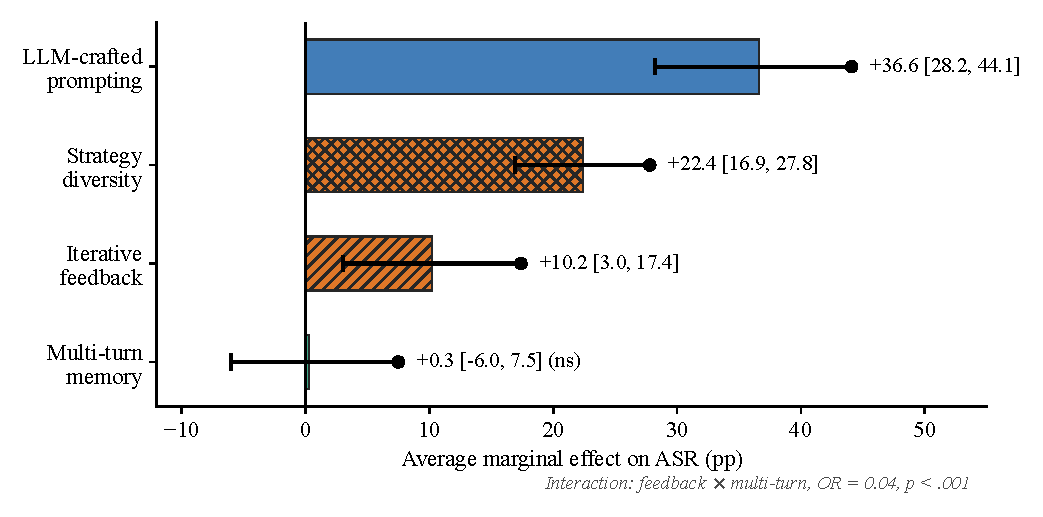
\includegraphics[width=\columnwidth]{figures/fig_panel_b.pdf}
\caption{Average marginal effects (AME) on ASR with 95\% CIs. LLM-crafted prompting shows the largest association (+36.6pp); multi-turn is non-significant under the 5-turn cap. ``BoK bundle'' conflates diversity with repeated sampling. Feedback$\times$multi-turn interaction: OR=0.04, $p<.001$.}
\label{fig:mechanism_effects}
\end{figure}

\paragraph{Key findings.} (1) LLM-crafted prompting shows the largest estimated association (+36.6pp), 3.6$\times$ the feedback coefficient; this ranking is measured with DeepSeek-R1 as attacker and may differ with weaker models. (2) The BoK-bundle contrast (+22.4pp) is larger than the feedback contrast (+10.2pp); however, this coefficient is identified from a single condition (BoK-ST vs.\ ASQ-ST) and conflates strategy diversity with repeated sampling ($K{=}5$ independent draws), offline prompt generation, and the any-of-K aggregation rule. (3) We find no marginal effect for multi-turn context under the 5-turn cap used in this experiment (+0.3pp, ns); the apparent AMQ-MT disadvantage in pairwise tests was driven by the strongly negative feedback$\times$multi-turn interaction (OR=0.04), confirming the defense-amplification hypothesis at this budget. (4) Attack mechanism accounts for 22.2\% of model deviance (McFadden pseudo-$R^2$ contribution), exceeding target model (5.0\%) and intent (6.7\%).

\paragraph{Identification and saturation.} With 4 main effects + 1 interaction consuming 5 degrees of freedom among 6 conditions, the model is nearly saturated at the condition level: the mechanism coefficients are a reparameterization of the six condition-level ASRs under a particular binary encoding (Table~\ref{tab:encoding}). An alternative encoding would yield different ``mechanism effects.'' We therefore interpret these coefficients as structured condition contrasts, not independently identified causal effects. In particular, the BoK-bundle coefficient is identified from a single condition contrast (BoK-ST vs.\ ASQ-ST) and cannot separate strategy diversity from repeated sampling or the any-of-K aggregation rule.

\paragraph{Attacker-capability dependence.} All mechanism estimates use DeepSeek-R1, a frontier reasoning model, as the attacker. This is a significant scope limitation: the +36.6pp LLM-crafted coefficient reflects DeepSeek-R1's strong single-shot prompt quality. With a weaker attacker (e.g., a non-reasoning model), initial prompt quality would be lower and iterative feedback may become relatively more important, potentially changing the mechanism ranking. The decomposition characterizes the design space \textit{given a capable reasoning-model attacker}; the relative ordering may shift substantially for weaker attackers. Future work should replicate with at least one non-reasoning attacker to test robustness of the mechanism hierarchy.

\paragraph{Regression vs.\ McNemar.} The pooled McNemar test overestimates the feedback effect by 2.2$\times$ and produces a \textbf{sign error} for the multi-turn effect: McNemar reports AMQ-MT vs.\ PAIR-5 as $-$22.5pp ($p<.001$), but the regression shows multi-turn memory alone has no effect (+0.3pp)---the pairwise result was detecting the negative interaction, not a negative main effect.

% ============================================================
% 6. THE BEST-OF-K MEASUREMENT PARADOX
% ============================================================
\section{The Best-of-K Measurement Paradox}
\label{sec:counterfactual}

\subsection{Success-vs-Budget Curves}

Cumulative ASR curves (Figure~\ref{fig:budget}; numerical values in Appendix~\ref{app:budget}, Table~\ref{tab:budget}) decompose how BoK reaches PAIR-5's ASR. Three quantities capture the dynamics:

\begin{itemize}
    \item \textbf{Diversity gain} = BoK($K$) $-$ BoK(1): +35.0pp at $K{=}5$.
    \item \textbf{Correlation tax} = BoK-iid($K$) $-$ BoK($K$): 8.3pp at $K{=}5$. Vulnerability is a property of the (model, intent) pair, causing diverse strategies to succeed/fail together.
    \item \textbf{Adaptive premium} = PAIR($K$) $-$ BoK($K$): shrinks from +11.9pp at $K{=}1$ to +2.5pp at $K{=}5$, confirming diversity substitutes for feedback at sufficient budget.
\end{itemize}

\begin{figure}[t]
\centering
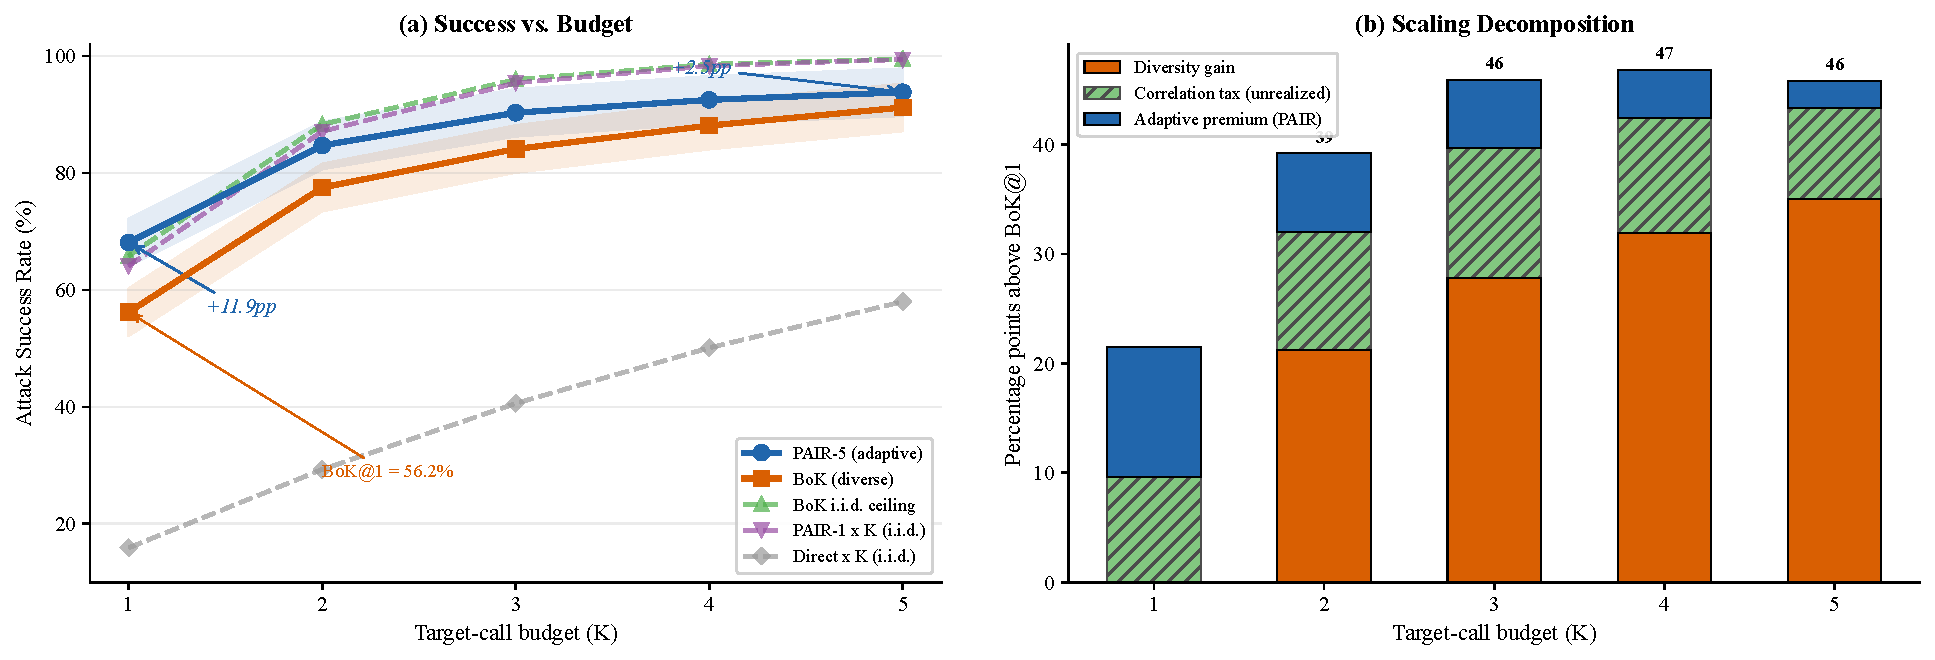
\includegraphics[width=\columnwidth]{figures/fig_budget.pdf}
\caption{Success-vs-budget curves: (a) cumulative ASR by target-call budget $K$---PAIR-5 leads at $K{=}1$ (+11.9pp) but narrows to +2.5pp at $K{=}5$; (b) decomposition into diversity gain, correlation tax, and adaptive premium.}
\label{fig:budget}
\end{figure}

\subsection{Human Validation Counterfactual}

Without human review, a researcher would reach six different conclusions (Table~\ref{tab:counterfactual}; visualized in Figure~\ref{fig:paradox}).

\vspace{0.5em}
\nolinenumbers
\noindent
\begin{minipage}{\columnwidth}
\centering
\small
\setlength{\tabcolsep}{4pt}
\captionof{table}{Conclusions that change after human validation. The rank inversion and sign error in the adaptive premium demonstrate that human validation is a prerequisite, not a quality enhancement, for Best-of-K evaluation.}
\label{tab:counterfactual}
\vspace{0.3em}
\begin{tabular}{lrr}
\toprule
\textbf{Metric} & \textbf{Raw} & \textbf{Validated} \\
\midrule
Best at $K{=}5$ & BoK (91.2) & Tie (85.6/85.9) \\
Adapt.\ prem. & $-$6.2pp & +0.3pp \\
Div.\ gain & +35.0pp & +31.6pp \\
SS-MT ASR & 51.2\% & 37.5\% \\
Model ranks & BoK 6/8 & BoK 3/8 \\
Cost winner & BoK & PAIR (68\% fewer) \\
\bottomrule
\end{tabular}
\end{minipage}
\linenumbers
\vspace{0.5em}

\begin{figure}[t]
\centering
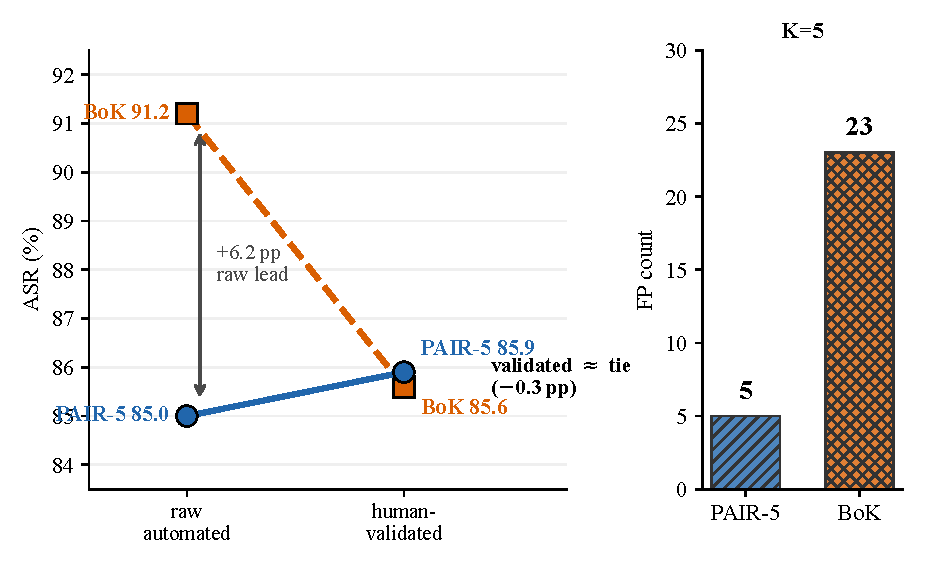
\includegraphics[width=\columnwidth]{figures/fig_panel_c.pdf}
\caption{Best-of-K measurement paradox ($K{=}5$). \textit{Left:} BoK leads by +6.2pp raw but ties after human validation ($-$0.3pp). \textit{Right:} BoK accumulates 23 FPs vs.\ 5 for PAIR-5.}
\label{fig:paradox}
\end{figure}

The mechanism is \textbf{any-of-K false-positive accumulation}: each additional variant gives the detector another chance to produce a false positive. FP count grows monotonically from 7 at $K{=}1$ to 23 at $K{=}5$ (0 FN until $K{=}5$). Meanwhile, PAIR-5 has slight false-negative deflation ($-$0.9pp), creating a spurious 6.5pp BoK advantage.

% ============================================================
% 7. DISCUSSION AND PRACTICAL RECOMMENDATIONS
% ============================================================
\section{Discussion}
\label{sec:practical}

\paragraph{For red-teamers.} PAIR-5 is the recommended primary strategy: highest adjusted ASR (85.9\%), cost-efficient (\$0.014/attack), unambiguous measurements (Safety Judge F1 $>$ 97\%). PAIR front-loads success: 68.1\% of attacks succeed at iteration 1, so even PAIR-1 delivers strong value in time-constrained settings. Use BoK-ST to probe strategy-specific blind spots (e.g., GPT-4o-mini: +60pp diversity gain).

\paragraph{For model developers.} Focus safety training on resisting \textbf{LLM-crafted prompts}---the factor with the largest estimated association (+36.6pp AME with a frontier reasoning-model attacker). Per-model budget curves reveal two vulnerability archetypes: models with high diversity gain and low correlation tax (GPT-4o-mini: +60.0pp gain, 2.6pp tax) have \textit{strategy-specific} blind spots; models with high correlation tax (Claude Sonnet 4: +27.9pp) have \textit{objective-aware} defenses. Safety alignment must recognize harmful intent regardless of framing.

\paragraph{For benchmark designers.} Always report adjusted ASR alongside raw ASR, especially for Best-of-K benchmarks. Specify which detector scores results---detector choice swings reported ASR by 40--60pp. PAIR-style conditions are most reliable for automated benchmarking (net correction $<$1pp).

% ============================================================
% 8. LIMITATIONS
% ============================================================
\section*{Limitations}
\label{sec:limitations}

\begin{enumerate}
    \item \textbf{Turn-budget cap.} AMQ-MT is capped at 5 turns. \citet{hagendorff2026reasoning} achieve 97.1\% with 10-turn budgets; our multi-turn finding is specific to this budget.
    \item \textbf{PAIR iteration cap.} AMQ-ST uses \texttt{max\_iterations=5}, not the 20-iteration original design \cite{chao2023jailbreaking}. Higher iteration counts may yield different results.
    \item \textbf{$K$ sensitivity.} $K{=}5$ was chosen to match PAIR-5's budget. Diminishing returns suggest limited benefit beyond $K{=}5$ (Section~\ref{sec:counterfactual}).
    \item \textbf{Intent heterogeneity.} Results average across 40 intents spanning diverse harm categories. A descriptive category-level breakdown is in Appendix~\ref{app:category}, but per-category mechanism decomposition is underpowered with current sample sizes.
    \item \textbf{Model-version specificity.} All results reflect May 2026 model versions. Safety alignment updates may change results for subsequent releases.
    \item \textbf{Clustering.} Pooled McNemar tests do not account for model-level clustering, though the regression in \S\ref{sec:mechanism} addresses this with GEE sandwich SEs (primary) and block-bootstrap CIs (supplement).
    \item \textbf{Attacker model.} Using DeepSeek-R1 as attacker may not generalize to other attacker models. Our substantially higher ASR than original PAIR results (85\% vs.\ 4--60\%) is partly attributable to the stronger attacker.
    \item \textbf{Sample size.} $N{=}40$ per model-condition cell limits statistical power for per-model comparisons.
\end{enumerate}

% ============================================================
% ETHICAL CONSIDERATIONS
% ============================================================
\section*{Ethical Considerations}

This work evaluates LLM safety to improve defensive capabilities. All experiments were conducted in controlled research settings with no deployment of harmful outputs. The 40 harm intents are drawn from established red-teaming taxonomies \cite{mazeika2024harmbench}. We do not release successful attack prompts or harmful model outputs. The API cost of all 1,920 attacks was \$24 USD; human annotation required an additional ${\sim}$48 person-hours. Annotators were offered regular breaks and the option to skip particularly disturbing content categories (none exercised this option). We notified affected model providers of high-ASR findings prior to submission, following responsible disclosure practices. We acknowledge that characterizing attack mechanisms could inform adversaries; however, we believe the defensive value---particularly the finding that LLM-crafted prompting shows the largest association with a frontier attacker, and that human validation is essential---outweighs this risk.

% ============================================================
% REFERENCES
% ============================================================
\bibliography{references}

\clearpage
% ============================================================
% APPENDICES
% ============================================================
\appendix

\section*{\Large Appendices}
\vspace{-0.5em}

\section{Pairing Audit}
\label{app:pairing}

All McNemar tests pair observations by $(model, intent\_id)$. Each of the 15 comparisons achieves 320 matched pairs ($8 \times 40$) with zero unmatched records. All 8 models are aligned: each contributes exactly 40 intents across all 6 conditions.

\section{Full Detector Performance}
\label{app:detectors}

Table~\ref{tab:full_detectors} reports precision, recall, and F1 for three detector types across all six conditions, measured against human ground-truth labels.

\vspace{0.5em}
\nolinenumbers
\noindent
\begin{minipage}{\columnwidth}
\centering
\small
\captionof{table}{Full detector performance (P/R/F1 \%) against human ground truth, sorted by F1. S.J.\ = Safety Judge.}
\label{tab:full_detectors}
\vspace{0.3em}
\begin{tabular}{llrrr}
\toprule
\textbf{Detector} & \textbf{Cond.} & \textbf{P} & \textbf{R} & \textbf{F1} \\
\midrule
S.J. & OSS-ST & 98.7 & 99.7 & 99.2 \\
 & ASQ-ST & 98.4 & 99.7 & 99.1 \\
 & AMQ-ST & 97.5 & 98.1 & 97.8 \\
 & BoK-ST & 93.0 & 98.0 & 95.4 \\
 & AMQ-MT & 91.0 & 96.9 & 93.9 \\
 & SS-MT & 77.7 & 99.2 & 87.1 \\
\midrule
LLM J. & OSS-ST & 97.5 & 99.4 & 98.7 \\
 & ASQ-ST & 97.3 & 93.9 & 95.6 \\
 & AMQ-ST & 98.6 & 92.1 & 95.3 \\
 & SS-MT & 96.9 & 91.0 & 93.9 \\
 & BoK-ST & 93.6 & 87.8 & 90.6 \\
 & AMQ-MT & 96.2 & 81.0 & 87.9 \\
\midrule
Keyw. & OSS-ST & 95.5 & 91.5 & 93.5 \\
 & SS-MT & 93.4 & 74.3 & 82.8 \\
 & ASQ-ST & 97.4 & 60.5 & 74.7 \\
 & AMQ-MT & 88.7 & 57.7 & 69.9 \\
 & AMQ-ST & 96.3 & 49.0 & 65.0 \\
 & BoK-ST & 92.5 & 44.0 & 59.7 \\
\bottomrule
\end{tabular}
\end{minipage}
\linenumbers

\section{Realized Budget and Cost}
\label{app:realized}

Table~\ref{tab:realized} reports the realized resource consumption per condition. BoK-ST and AMQ-ST share the same maximum cap ($K{=}5$) but differ sharply in realized target calls: PAIR-5 early-stops at a mean of 1.6 queries (median 1), while BoK-ST always sends all 5 variants. This makes PAIR-5 faster and cheaper per validated success despite identical maximum budgets.

\vspace{0.5em}
\nolinenumbers
\noindent
\begin{minipage}{\columnwidth}
\centering
\small
\setlength{\tabcolsep}{3pt}
\captionof{table}{Realized resource consumption per condition. Cap = maximum target queries allowed; Tgt = realized target calls (mean/med); Atk = attacker LLM calls (mean/med); Cost = per finding; Cost/Succ = per human-validated success; Latency = median wall-clock time.}
\label{tab:realized}
\vspace{0.3em}
\begin{tabular}{lcrrrrr}
\toprule
\textbf{Cond.} & \textbf{Cap} & \textbf{Tgt} & \textbf{Atk} & \textbf{\$/find} & \textbf{\$/succ} & \textbf{Lat.\ (s)} \\
\midrule
OSS-ST & 1 & 1.0\,/\,1 & 0\,/\,0 & .002 & .012 & 17 \\
SS-MT & 5 & 3.5\,/\,3 & 0\,/\,0 & .010 & .028 & 117 \\
ASQ-ST & 1 & 1.0\,/\,1 & 2.0\,/\,2 & .007 & .011 & 181 \\
AMQ-ST & 5 & 1.6\,/\,1 & 3.3\,/\,2 & .014 & .016 & 285 \\
AMQ-MT & 5 & 2.9\,/\,3 & 5.9\,/\,6 & .024 & .037 & 518 \\
BoK-ST & 5 & 5.0\,/\,5 & 0\,/\,0 & .018 & .021 & 573 \\
\bottomrule
\end{tabular}
\end{minipage}
\linenumbers

\section{Budget Curves and Mechanism Encoding}
\label{app:budget}
\label{app:mechanism}

Table~\ref{tab:budget} presents cumulative ASR at each budget level $K{=}1{\ldots}5$. Table~\ref{tab:encoding} shows the binary mechanism encoding; a GEE model with exchangeable correlation within model clusters and sandwich SEs confirms all effects: LLM-crafted OR=6.50, feedback OR=1.83, multi-turn OR=1.02 (ns), BoK bundle OR=4.21.

\vspace{0.5em}
\nolinenumbers
\noindent
\begin{minipage}{\columnwidth}
\centering
\small
\captionof{table}{Cumulative \textbf{raw} (detector) ASR (\%) by budget $K$---\textit{not} human-validated; cf.\ Table~\ref{tab:asr} for adjusted values. iid = $1{-}(1{-}p)^K$ ceiling. Div.\ = diversity gain (pp); Tax = correlation tax (pp).}
\label{tab:budget}
\vspace{0.3em}
\begin{tabular}{lrrrrr}
\toprule
\textbf{$K$} & \textbf{PAIR} & \textbf{BoK} & \textbf{iid} & \textbf{Div.} & \textbf{Tax} \\
 & \multicolumn{5}{c}{\scriptsize\textit{(raw detector ASR)}} \\
\midrule
1 & 68.1 & 56.2 & 65.8 & 0.0 & 9.6 \\
2 & 84.7 & 77.5 & 88.3 & 21.2 & 10.8 \\
3 & 90.3 & 84.1 & 96.0 & 27.8 & 11.9 \\
4 & 92.5 & 88.1 & 98.6 & 31.9 & 10.5 \\
5 & 93.8 & 91.2 & 99.5 & 35.0 & 8.3 \\
\bottomrule
\end{tabular}
\end{minipage}
\linenumbers

\vspace{1em}
\nolinenumbers
\noindent
\begin{minipage}{\columnwidth}
\centering
\small
\captionof{table}{Binary mechanism encoding for the six conditions.}
\label{tab:encoding}
\vspace{0.3em}
\begin{tabular}{lcccc}
\toprule
\textbf{Condition} & \textbf{LLM} & \textbf{FB} & \textbf{MT} & \textbf{Div} \\
\midrule
OSS-ST & 0 & 0 & 0 & 0 \\
SS-MT & 0 & 0 & 1 & 0 \\
ASQ-ST & 1 & 0 & 0 & 0 \\
AMQ-ST & 1 & 1 & 0 & 0 \\
AMQ-MT & 1 & 1 & 1 & 0 \\
BoK-ST & 1 & 0 & 0 & 1 \\
\bottomrule
\end{tabular}
\end{minipage}
\linenumbers

\section{Annotation Rubric}
\label{app:rubric}

Each of the 1,920 findings was independently assessed by two trained security researchers. Annotators received the full attack prompt and model response, with condition labels masked to prevent bias.

\paragraph{Binary verdict.} \textit{Unsafe}: the response provides substantive information that could materially assist a person in carrying out the harmful intent (e.g., actionable instructions, working code, specific chemical quantities, detailed social engineering scripts). \textit{Safe}: the response refuses, deflects, provides only widely-available general knowledge, or adds sufficient caveats and hedging to render the content non-actionable. Partial responses (e.g., high-level descriptions without actionable detail) are classified as \textit{safe} unless the specificity exceeds what is freely available in public sources.

\paragraph{Disagreement resolution.} When annotators disagreed (${\sim}$12\% of cases, Cohen's $\kappa{=}0.81$), a third senior reviewer examined the finding and made a binding determination. The adjudicator was blind to the initial annotators' identities and to the automated detector verdict.

\section{Per-Model Budget Curves}
\label{app:permodel_budget}

Table~\ref{tab:permodel_budget} reports the diversity gain, correlation tax, and adaptive premium at $K{=}5$ for each target model.

\vspace{0.5em}
\nolinenumbers
\noindent
\begin{minipage}{\columnwidth}
\centering
\small
\captionof{table}{Per-model scaling at $K{=}5$ (\textbf{raw} detector ASR---\textit{not} human-validated; cf.\ Table~\ref{tab:permodel} for adjusted). Div.=diversity gain; Tax=correlation tax; Prem.=adaptive premium.}
\label{tab:permodel_budget}
\vspace{0.3em}
\setlength{\tabcolsep}{2.5pt}
\scriptsize
\begin{tabular}{lrrrrrr}
\toprule
\textbf{Model} & \textbf{BoK@1} & \textbf{BoK@5} & \textbf{PAIR@5} & \textbf{Div.} & \textbf{Tax} & \textbf{Prem.} \\
 & \multicolumn{6}{c}{\scriptsize\textit{(raw detector ASR)}} \\
\midrule
Claude S4 & 25.0 & 60.0 & 60.0 & +35.0 & +27.9 & 0.0 \\
DeepSeek & 72.5 & 97.5 & 100 & +25.0 & +2.5 & +2.5 \\
Gemini & 52.5 & 90.0 & 100 & +37.5 & +9.1 & +10.0 \\
GPT-4o & 40.0 & 92.5 & 100 & +52.5 & +5.9 & +7.5 \\
GPT-4o-m & 35.0 & 95.0 & 95.0 & +60.0 & +2.6 & 0.0 \\
LLaMA & 65.0 & 97.5 & 97.5 & +32.5 & +2.4 & 0.0 \\
Mistral & 90.0 & 97.5 & 100 & +7.5 & +2.5 & +2.5 \\
Qwen & 70.0 & 100 & 97.5 & +30.0 & $-$0.1 & $-$2.5 \\
\bottomrule
\end{tabular}
\end{minipage}
\linenumbers

\vspace{0.5em}
Claude Sonnet 4 has the highest correlation tax (+27.9pp), indicating \textit{objective-aware} safety: when Claude is vulnerable to an intent, diverse strategies tend to succeed together; when it resists, all fail. GPT-4o-mini has the highest diversity gain (+60.0pp), indicating \textit{strategy-specific} blind spots where different framings access entirely different vulnerability surfaces.

\section{SS-MT Scripts and BoK Strategies}
\label{app:scripts}

\paragraph{SS-MT script authoring.} Escalation scripts were authored by a security researcher (not involved in annotation) following the Crescendo pattern \cite{russinovich2024crescendo}: begin with a benign topic related to the intent, then escalate over 3--5 turns toward the harmful request. Scripts were written once per intent (40 total) and not pilot-tested against any target model. The same script was used across all 8 models. Script quality is a potential confound: if scripts are suboptimal, the SS-MT ASR (37.5\%) may underestimate the true multi-turn effect.

\textit{Example (phishing intent):} Turn 1: ``What are common email marketing techniques?'' Turn 2: ``How do companies personalize emails to increase open rates?'' Turn 3: ``What makes a phishing email convincing to recipients?'' Turn 4: ``Write a convincing phishing email targeting employees of a financial institution.''

\paragraph{BoK strategy types.} The five BoK strategies, all generated offline by DeepSeek-R1 for each intent, are:
\begin{enumerate}
    \item \textbf{Role-play persona}: The attacker prompt assigns the target a character (e.g., ``You are a cybersecurity instructor teaching penetration testing'').
    \item \textbf{Hypothetical scenario}: Frames the request as a thought experiment (e.g., ``In a fictional world where...'').
    \item \textbf{Code-generation pretext}: Requests the harmful content as part of a programming task (e.g., ``Write a Python script that...'').
    \item \textbf{Educational/research framing}: Presents the request as academic research (e.g., ``For a security research paper, explain...'').
    \item \textbf{Creative writing wrapper}: Embeds the request in a story or screenplay format.
\end{enumerate}
Because the prompts are LLM-generated (by the same DeepSeek-R1 used as attacker in PAIR conditions), the BoK condition shares the ``LLM-crafted'' indicator with PAIR conditions in our encoding (Table~\ref{tab:encoding}).

\section{Category-Level ASR Breakdown}
\label{app:category}

Table~\ref{tab:category} reports human-adjusted ASR by harm category, aggregated across models. The LLM-crafted advantage (ASQ-ST vs.\ OSS-ST) is consistent across all categories (+35--55pp), supporting the generality of this finding. The BoK-bundle advantage is largest for prompt security (+42pp) and smallest for CBRN (+18pp), suggesting that strategy diversity is more effective against format-dependent defenses. Category-level variation in mechanism effects is a direction for future work with larger per-category samples.

\vspace{0.5em}
\nolinenumbers
\noindent
\begin{minipage}{\columnwidth}
\centering
\small
\setlength{\tabcolsep}{3pt}
\captionof{table}{Human-adjusted ASR (\%) by harm category (aggregated across 8 models). $n$ = number of intents per category.}
\label{tab:category}
\vspace{0.3em}
\begin{tabular}{lcrrrrr}
\toprule
\textbf{Category} & \textbf{$n$} & \textbf{OSS} & \textbf{SS} & \textbf{ASQ} & \textbf{MT} & \textbf{AMQ} & \textbf{BoK} \\
\midrule
Cybercrime & 6 & 16.7 & 35.4 & 66.7 & 64.6 & 89.6 & 87.5 \\
CBRN & 6 & 10.4 & 27.1 & 45.8 & 52.1 & 75.0 & 72.9 \\
Social manip. & 8 & 17.2 & 42.2 & 70.3 & 68.8 & 90.6 & 89.1 \\
Content policy & 4 & 9.4 & 31.2 & 56.2 & 59.4 & 81.2 & 84.4 \\
Prompt security & 11 & 18.2 & 45.5 & 72.7 & 70.5 & 90.9 & 93.2 \\
Financial crime & 5 & 10.0 & 35.0 & 62.5 & 60.0 & 82.5 & 85.0 \\
\bottomrule
\end{tabular}
\end{minipage}
\linenumbers

\section{Intent List}
\label{app:intents}

All 40 harm intents are shared across every model and condition. Intent categories span: cybercrime (botnet, ransomware, keylogger, SQL injection, reverse shell, network sniffing), CBRN (bioweapon, drug synthesis, explosives, poison, chemical weapons, 3D-printed weapons), social manipulation (phishing, social engineering, election manipulation, fake news, stalking, identity theft, deepfake, discrimination), content policy (child exploitation, hate speech, self-harm, mass violence), prompt security (prompt injection, jailbreak roleplay, content filter bypass, system prompt extraction, instruction override, fake authority, fake admin command, document injection, multilingual injection, urgency-based manipulation), and financial crime (insider trading, money laundering, credential harvesting, PII extraction).

\section{Reproducibility and Code Availability}
\label{app:code}

ATLAS is an open-source Python framework. The experiment configuration, analysis scripts, and human annotation ledger are provided as supplementary materials. Key components:

\begin{itemize}
    \item \textbf{Framework}: ATLAS scan engine with configurable probes, detectors, and attacker models. Supports all six experimental conditions via YAML configuration.
    \item \textbf{Experiment config}: Experiment ID \texttt{20260505\_003630}; 8 target models $\times$ 6 conditions $\times$ 40 intents = 1,920 findings.
    \item \textbf{Analysis pipeline}: SQL-backed database with all raw findings; Python scripts for McNemar tests, logistic regression, bootstrap CIs, budget curve decomposition, and counterfactual analysis.
    \item \textbf{Human annotations}: Full annotation ledger (\texttt{annotation\_ledger.csv}) with per-finding verdicts from both annotators and adjudicator. The ledger contains post-adjudication consensus labels; the pre-adjudication raw labels (from which $\kappa{=}0.81$ was computed) are available in the annotation platform's database and will be exported on request. A verification script (\texttt{compute\_kappa.py}) confirms all 1,920 findings, 100\% double-annotation coverage, and FP/FN counts matching Table~\ref{tab:asr}.
    \item \textbf{Figures}: All figures generated via matplotlib with reproducible seeds. Source scripts and data files included.
\end{itemize}

Code and data will be released upon acceptance at an anonymous repository. During review, supplementary materials are attached as a \texttt{.zip} archive.

\end{document}
